
\section{Social Graph}

In social graph, we often want to extract communities, use clustering


Strong and weak communities, for a given vertex $i$ we define

\begin{itemize}
  \item the internal degree $k_i^{int}$ the number of edges from $i$ going to another vertex of the community
  \item the external degree $k_i^{ext}$ the number of edges from $i$ going to a vertex outside of the community
\end{itemize}

$k_i^{int}$ should be high and $k_i^{ext}$ should be low, otherwise change the community. We should have

\[
  \sum_{i\in C} k_i^{int}(C) > \sum_{i\in C} k_i^{out}(C)
\]

Community detection

We build a similarity matrix ($A_{ij}$ how node $i$ and $j$ are similar) from the adjacency matrix.

Hierarchical clustering identifies groups of nodes with high similarity. Two strategies:

\begin{itemize}
  \item agglomerative algorithm: merge nodes and communities with high similarity
  \item divisive algorithm: split communities by removing links connecting nodes with low similarity (smallest cut)
\end{itemize}

Keep the historic for a choice or chose the $k$ number of communities.

Finding a weak edge

\begin{definition}[Edge betweenness]
  Number of shortest paths passing over an edge ($O(n^2)$)
\end{definition}

Girvan-Newman method: divisive hierarchical clustering based on edge betweenness. Iteratively remove edge of highest betweenness. Complexity $O(ln^2)$, $O(n^3)$ for sparse graph.


\begin{definition}[Random walk betweenness]
  Given two nodes $i$ and $j$, $x_{ij}$ is the probability that the edge between $i$ and $j$ is taken by a walk averaged over all the random walks between the pairs of node of the graph.
\end{definition}

How to compute betweenness ? repeat for each node, but let's say $A$ w.l.o.g. see \cref{fig:betweenness}

\begin{itemize}
  \item BFS from node $A$, all nodes are layered
  \item For each node $i$, count the number of shortest paths arriving to $i$. Recursively sum up the count of the parent layer connected nodes (assigning 1 to node $A$).
  \item Assign edge value bottom up, each node has value $1 + \sum $ child edges, to distribute proportionally to its parents (according to their weight)
\end{itemize}

\begin{definition}[Modularity]
  Modularity measures how well a network is partitioned into communities and is defined by 
  \[
    Q \propto \sum_{s \in S} (\text{\# edges within } s) - (expected \text{\# edges within } s)
  \]
  with $S$ a family of set of vertex partitioning the graph. The second part of the sum is computed on a graph with same degree distribution but random connections (null model).
\end{definition}


\begin{definition}[Normalized modularity]
  For a given graph $G$ and a partitioning $S$
  \[
    Q(G,S) = \underbrace{\frac 1 {2m}}_{\text{normalize}} \sum_{s\in S, i,j\in s} \l(A_{ij} - \frac{k_ik_j}{2m}\r)
  \]
  and $-1<Q<1$
\end{definition}

Modularity is positive if the intra connection exceeds the expected number, significant if $Q>0.3,0.7$. Use modularity to know when to stop partitioning (pick).

\begin{figure}
  \centering
  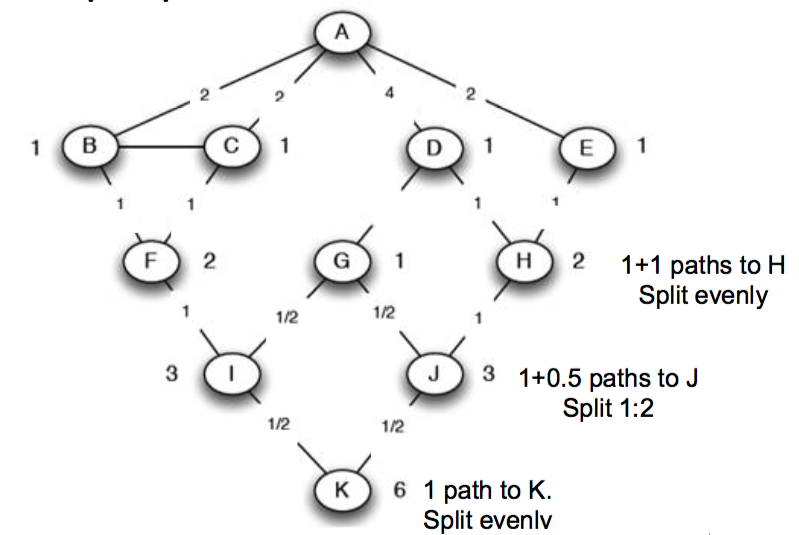
\includegraphics[width=1\linewidth]{figures/betweenness_computation.png}
  \caption{Betweenness computation - BFS, top down node weighting, bottom up edge values}
  \label{fig:betweenness}
\end{figure}

Louvain Modularity: greedy optimization in $O(n\log n)$, find small communities locally and then group smallest communities as simple nodes

\begin{definition}[Small world graphs]
  Graph for which most nodes are not neighbors of one another but most nodes can be reached from any other node by a small number of hops
\end{definition}

Milgram's experiment: message from Nebraska to Massachusetts, from people to people (mean of 5-6 hopes)

Random graph
\begin{itemize}
  \item low diameter, expected distance between two nodes is $\log_k n$ with $k$ the average outdegree
  \item a pair $(i,j) \in V^2$ picked uniformly at random is connected by a short path with high probability
  \item low clustering coefficient (inaccurate for social graph modeling)
\end{itemize}

\begin{definition}[diameter]
  The diameter of a graph $G$ is the longest shortest path between any pair of nodes.
\end{definition}

\begin{definition}[Local clustering coefficient]
  The local clustering coefficient is the proportion of neighbors connected for a given node. Formally for a given edge $i$ with neighbors $N$ and edges between them $E$
  \[
    C_i = \frac { 2|E|}{|N|(|N|-1)}
  \]
\end{definition}


% Random rewiring of regular graph (by Watts and Strogatz): with probability $p$ rewire each link in a regular graph to a randomly selected node. Resulting graph has properties, both of regular and random graphs, see \cref{fig:watts_strogatz}.

\begin{figure}
  \centering
  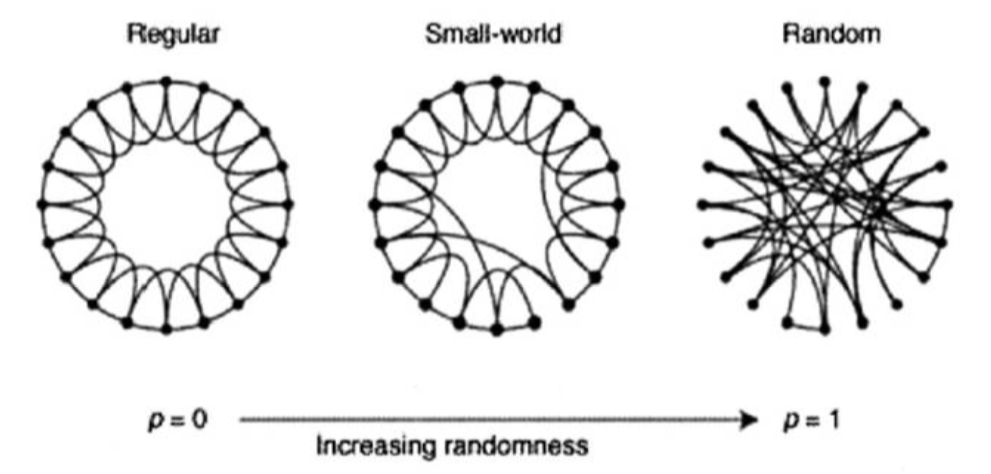
\includegraphics[width=1\linewidth]{figures/watts_strogatz_graph.png}
  \caption{Watts Strogatz rewiring construction}
  \label{fig:watts_strogatz}
\end{figure}

Efficient search algorithm

Kleinberg’s Small-World Model
\begin{itemize}
  \item Embed a graph into an $d$-dimensional grid to define a distance ($l-2$ norm for instance)
  \item each node is connected to $p$ of its closest neighbor (short range links) + $q$ long range links according to a distribution
  \[
    \P{u \leftrightarrow v} \propto \text{dist}(u,v)^{-r}
  \]
\end{itemize}

Decentralized routing algorithm performs well iff $r=$ dimension of the space.

$r=0$ uniform choice, there exist short paths between every pair of vertices picked uniformely, but there is no decentralized algorithm capable finding these paths efficiently

$r$ too small, we go far but struggle to converge, $r$ too high we stay among our neighbors, hard to go far.

Routing cost: with $O(1)$ long range link $O(\log^2 n)$, and with $O(\log n)$ long range links $O(\log n)$
